\documentclass[a4paper,11 pt]{article}
\usepackage[utf8]{inputenc}
\UseRawInputEncoding
%\usepackage[spanish]{babel}
\usepackage [pdftex]{graphicx}
%\parindent 
\begin{document}
\title {Pumped Hydraulic Storage }
\author{Francisco José Martínez Sáez}
\date{22/10/2019}
\maketitle
\begin{abstract}
URL del repositorio
\end{abstract}


\section {Keywords of the article}
{\bf Keywords:} Pumped-storage hydroelectricity, , pumped hydraulic storage, hydraulic storage pumped, electrical energy.

\section {Introduction}
There are many forms of mechanical energy storage, for example, compressed air energy storage, fireless locomotive, flywheel energy storage, gravitational potential energy or hydraulic accumulator. However, let's now focus on one of the most important types of energy storage that currently exist, pumped-storage hydroelectricity.

\section {State of the art}
Traditionally, pumped hydraulic storage has been used in coal and nuclear power plants. The demand for energy is fluctuating and this increases production peaks to reach that demand. This causes a decrease in the performance and efficiency of the plant. Through the hydraulic storage pumped, the energy is stored in the hours of low consumption and can be used in the hours of high demand, allowing an optimal and continuous production of energy. \cite{Wilson2018}\\ \\
However, with the growth of clean energies, a new use appears for pumped-storage hydroelectricity. As already mentioned, renewable energy sources such as solar and wind energy depend on environmental variables beyond the reach of humans (they are intermittent energy sources). Pumped-storage hydroelectricity allows generating energy at a time of high production (more energy is produced than consumed) and using it in another time of low production to meet the demand regardless of the weather conditions and specific demand. \cite{Roca2017} \cite{Wilson2018}\\ \\


\begin {figure}[h]
\begin{center}
\includegraphics[width=80mm,height=50mm]{photo2.jpg}
\caption {Shaded-relief topo map of the Taum Sauk pumped storage plant in Missouri}
\end{center}
\end{figure}


The principle of storage by pumping is to use the gravitational potential to store energy. There are two water tanks, one higher than the other, and a system of pipes that connect them.  Inside the pipes there is a reversible motor / turbine system. When the demand is low and there is an excess of energy production (weekends or at night) the plant uses energy to pump water from the lower tank to the upper tank. When the demand is high and more energy is needed than what is being produced, the water from the upper reservoir returns to the lower one through the same piping system, the potential energy of the water passes to kinetic energy and when it passes through the turbines it transforms in rotating mechanical energy. Finally, high and medium voltage electrical energy is obtained in the generator.  \cite{Lewis2017} \cite{Roca2017} \\ \\


\begin {figure}[h]
\begin{center}
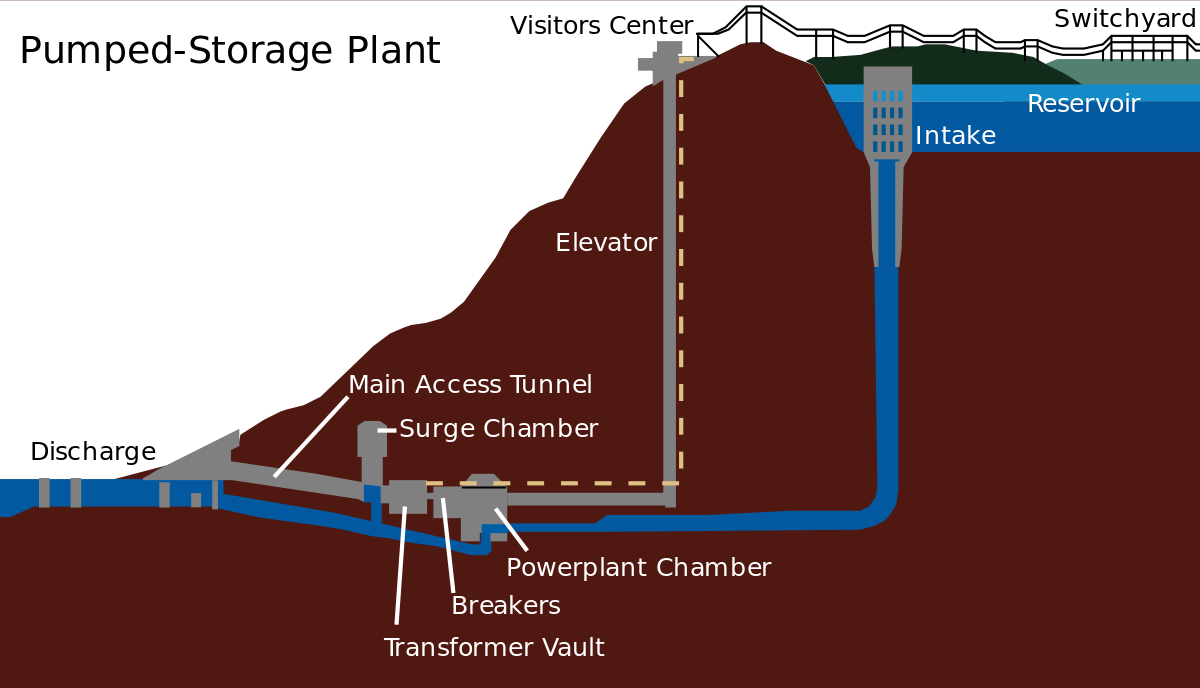
\includegraphics[width=80mm,height=50mm]{photo.png}
\caption {Operation of a pumped-storage hydroelectricity plant}
\end{center}
\end{figure}

\begin {displaymath}
E= P\cdot t 
\end {displaymath}
\begin {displaymath}
Egenerador= \rho \cdot g \cdot h \cdot V \cdot \mu
\end {displaymath}
\begin {displaymath}
Ebomba= (\rho \cdot g \cdot h \cdot V)/ \mu
\end {displaymath}

\parskip= 4 cm
\parindent 0 cm
The largest pumped-storage hydroelectricity plant in the world is Bath County Central, in the USA. It was completed in 1985 at a cost of 1,600 million dollars and has a generation capacity of 3003 MW. [5]\\\\
The largest power station in Europe and the eighth largest in the world is the Grand'Maison Central, in France. It has a power generation capacity of 1800 MW. \cite{Lewis2017} \\ \\

\parskip= 1 cm
\parindent 0 cm
\begin{tabular}{|c||c||c|}
\hline \multicolumn {3}{|c|}{The largest pumped-storage hydroelectricity plants in the world}\\
\hline Central & Country & Storage capacity\\
\hline Bath County Central & USA & 3003 MW\\
\hline Guangdong Pumped Storage Power Station & China & 2400 MW\\
\hline Huizhou Pumped Storage Power Station &	China & 2400 MW\\
\hline
\end {tabular}

\parskip= 1 cm
\parindent 1 cm
Taking into account the evaporative losses of the surface of the exposed water and the losses by conversion, an energy recovery of 70-80\% or more can be achieved, therefore, it is the energy storage form of the larger capacity network available according to the global energy storage database of the United States Department of Energy. However, the environmental impact of a plant of this type is very high; in addition, the high initial cost and construction time are some drawbacks of this interesting form of energy storage. \cite{Boysen2018} \\\\

\bibliography{BaseDeDatos}
\bibliographystyle{plain}

\begin{thebibliography}{1}

\bibitem{Boysen2018}
Angie Boysen.
\newblock Pumped storage hydroelectricity.
\newblock {\em Stanford University}, 2018.

\bibitem{Lewis2017}
Lewis.
\newblock Pumped storage hydro plants.
\newblock {\em Duke Energy}, 2017.

\bibitem{Roca2017}
Jose~Antonio Roca.
\newblock Las 10 mayores centrales hidroeléctricas de bombeo del mundo.
\newblock {\em el periodico de la energía}, 2017.

\bibitem{Wilson2018}
Wilson.
\newblock Pumped hydropower.
\newblock {\em Energy Storage Association}, 2018.

\end{thebibliography}




\end{document}